%\section{Data Model}
%
%
%\subsection{Smart Contract for Event Hosting}
%The class diagram in Figure \ref{fig:event-data-model} illustrates how events are created and registered, tickets can be issued and distributed. Important to %point out is that a presale only makes sense for fungible tickets. 
%\begin{figure}[H]
%    \centering
%    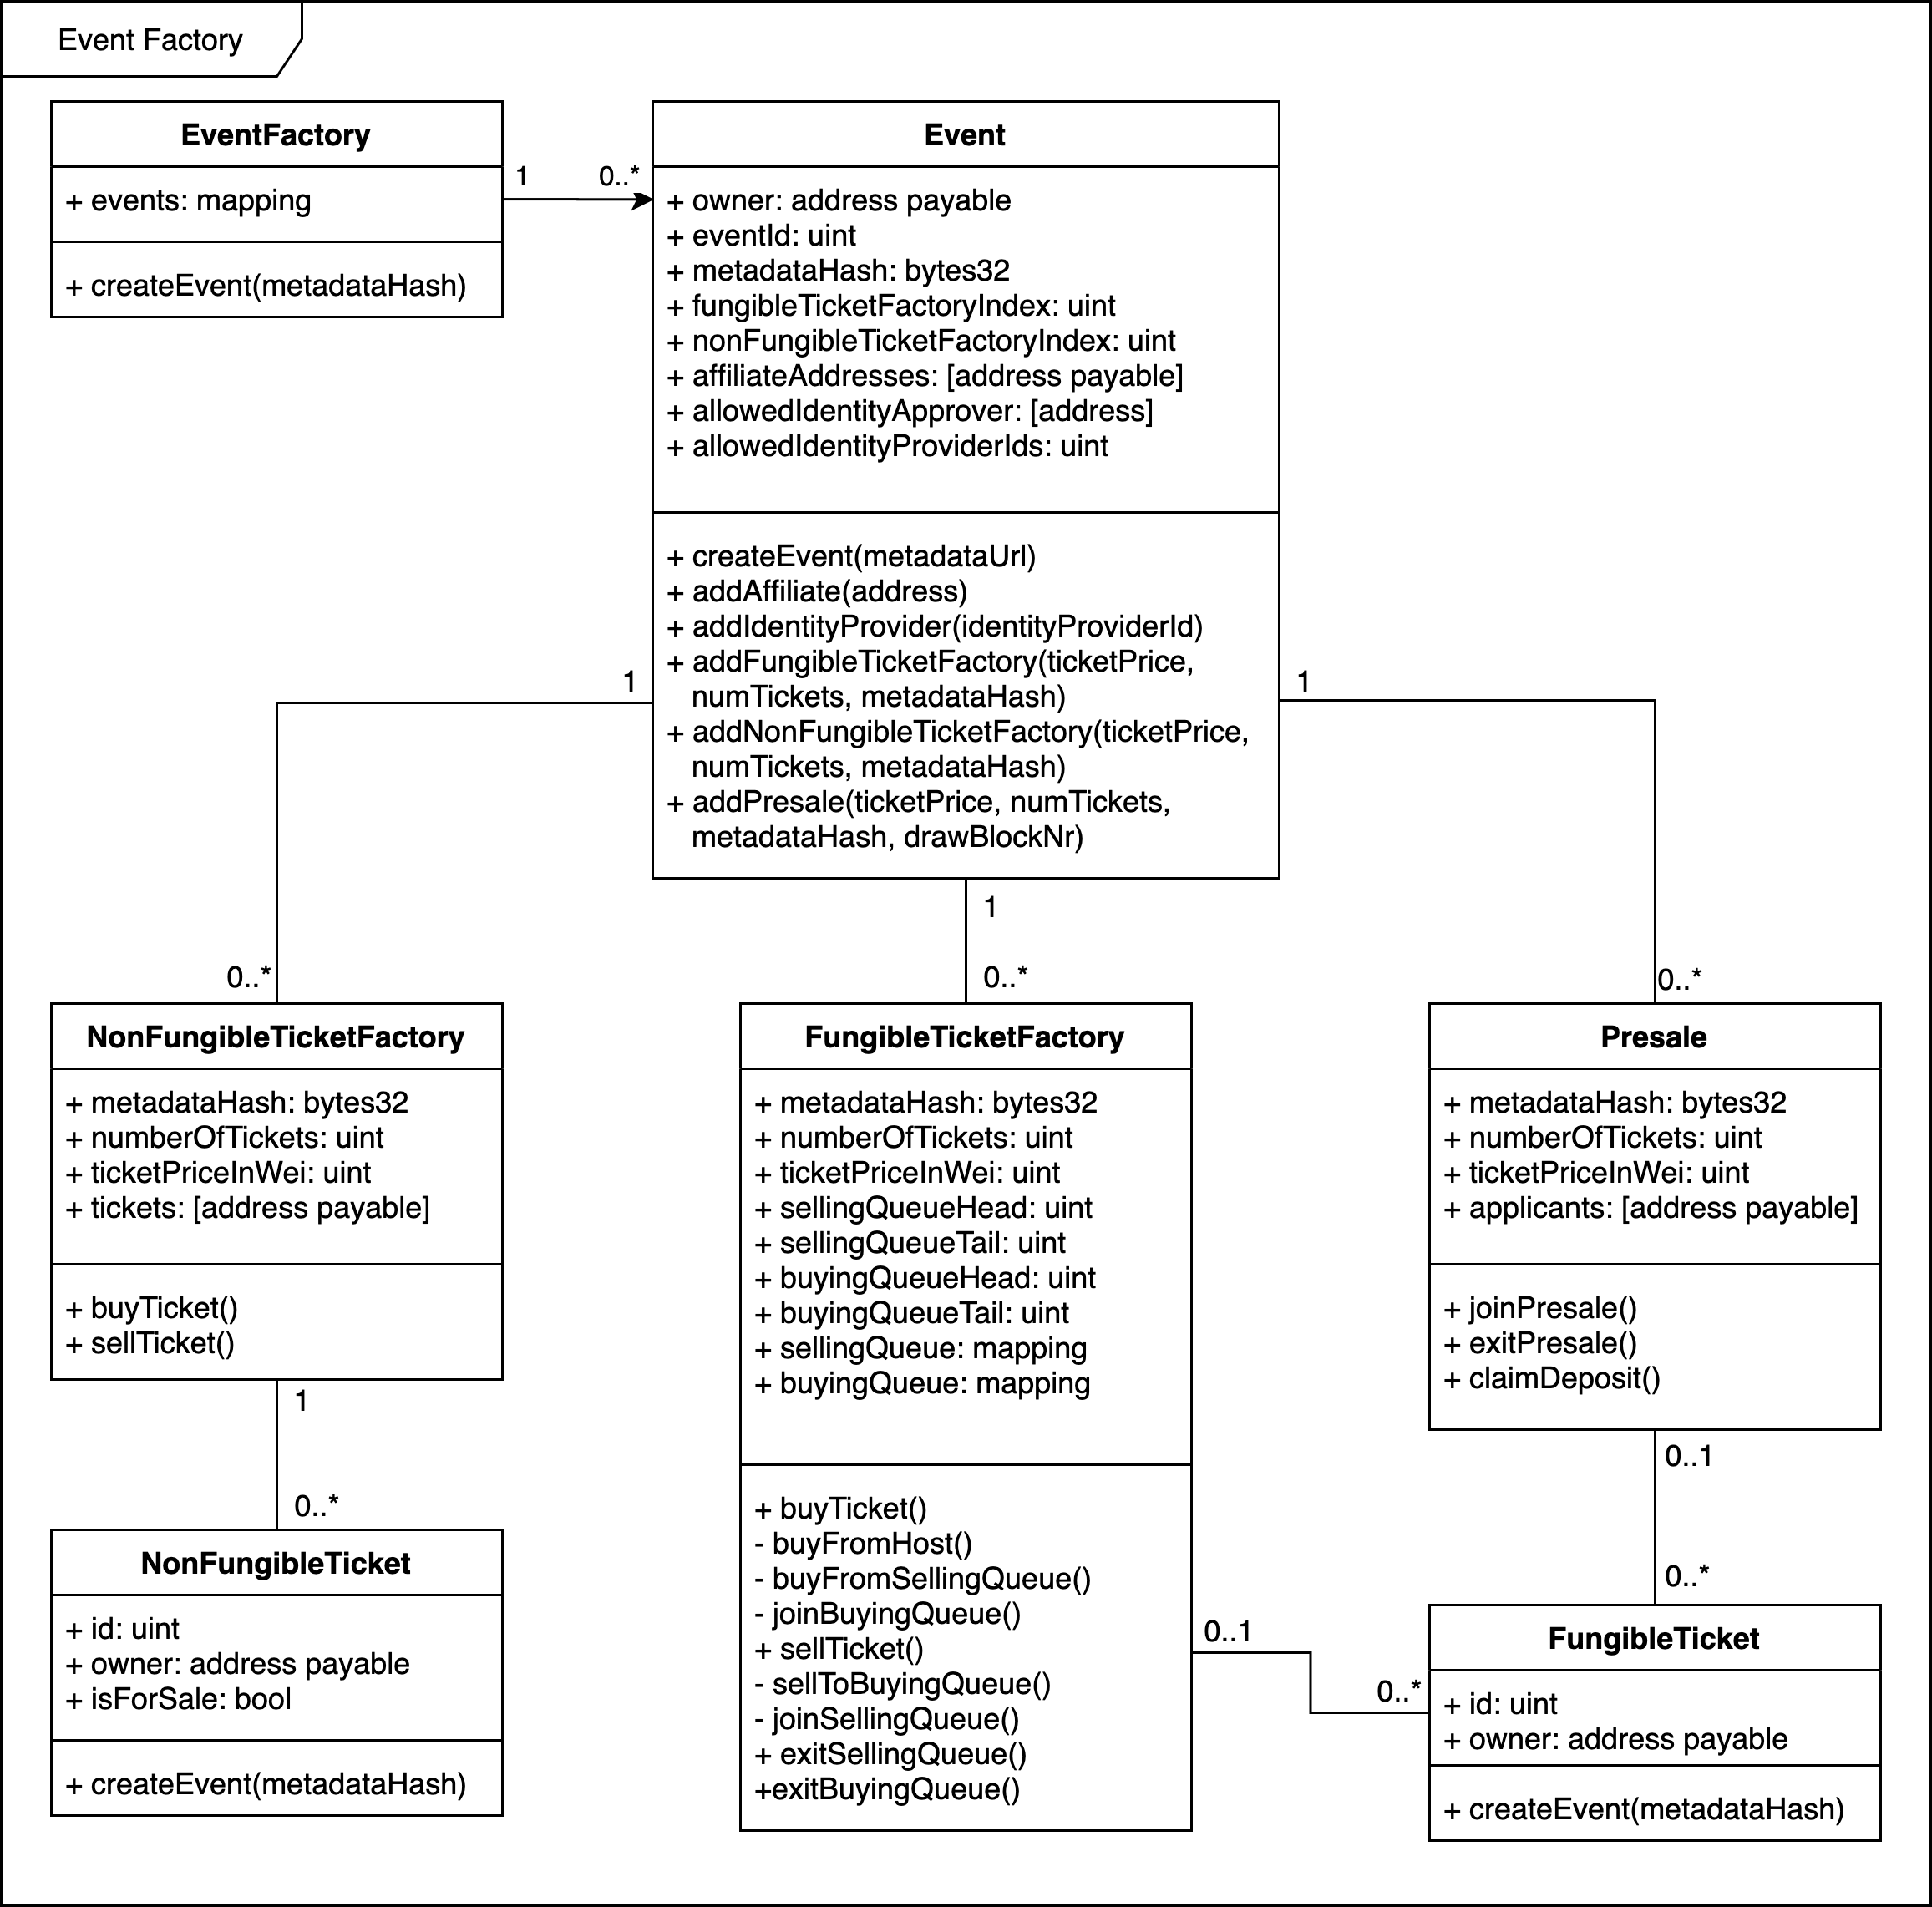
\includegraphics[width=16cm]{design/diagrams/event-factory-class-diagramm.png}
%    \caption{Event Data Model}
%    \label{fig:event-data-model}
%\end{figure}
\begin{comment}
\subsection{Smart Contract for Identity Registration}

\subsection{RESTful Service for Identity Registration and Approval}
To interact with the identity approver, a Rest API as in Table \ref{tab:Identity-Reg-Rest-API} is used. The first step is to register an identity for approval. A secret will then be sent to this identity. In the next step, the identity is validated using the ETHadress and the secret received.

\begin{table}[H]
\caption{Identity Registration and Approval Rest API}
\label{tab:Identity-Reg-Rest-API}

\begin{tabular} { | m{0.3\textwidth} |m{0.1\textwidth}|m{0.2\textwidth}|m{0.2\textwidth} | }
\hline
Mapping & Type & Parameters & Return \\
\hline
  /addEmailIdentity & Post & eMail & boolean \\ 
\hline
/validateEmailIdentity & Post & eMail  & EmailIdentity \\ 
& &secret  & \\
& & signedSecret  & \\
& & ethAddress & \\
\hline
/addPhoneIdentity   & Post & phoneNr & boolean \\ 
\hline
/validatePhoneIdentity & Post & phoneNr & PhoneIdentity \\ 
& &secret  & \\
& & signedSecret  & \\
& & ethAddress & \\
\hline
\end{tabular}

\end{table}


\subsection{RESTful Service for Access Control}
\end{comment}